% !TEX TS-program = pdflatex
% !TEX encoding = UTF-8 Unicode

% This file is a template using the "beamer" package to create slides for a talk or presentation
% - Talk at a conference/colloquium.
% - Talk length is about 20min.
% - Style is ornate.

% MODIFIED by Jonathan Kew, 2008-07-06
% The header comments and encoding in this file were modified for inclusion with TeXworks.
% The content is otherwise unchanged from the original distributed with the beamer package.

\documentclass{beamer}


% Copyright 2004 by Till Tantau <tantau@users.sourceforge.net>.
%
% In principle, this file can be redistributed and/or modified under
% the terms of the GNU Public License, version 2.
%
% However, this file is supposed to be a template to be modified
% for your own needs. For this reason, if you use this file as a
% template and not specifically distribute it as part of a another
% package/program, I grant the extra permission to freely copy and
% modify this file as you see fit and even to delete this copyright
% notice. 


\mode<presentation>
{
  \usetheme{Warsaw}
  % or ...

  \setbeamercovered{transparent}
  % or whatever (possibly just delete it)
}


\usepackage[english]{babel}
% or whatever

\usepackage[utf8]{inputenc}
% or whatever

\usepackage{times}
\usepackage[T1]{fontenc}
% Or whatever. Note that the encoding and the font should match. If T1
% does not look nice, try deleting the line with the fontenc.


\title[Short Paper Title] % (optional, use only with long paper titles)
{Prediction of a Connectome Based on Fluorescence Data}

%\subtitle
%{Include Only If Paper Has a Subtitle}

\author % (optional, use only with lots of authors)
{Guy W. Cole, Isaiah S. Morales, Austin Stone}
% - Give the names in the same order as the appear in the paper.
% - Use the \inst{?} command only if the authors have different
%   affiliation.

%\institute[Universities of Somewhere and Elsewhere] % (optional, but mostly needed)
%{
%  \inst{1}%
%  Department of Computer Science\\
%  University of Somewhere
%  \and
%  \inst{2}%
%  Department of Theoretical Philosophy\\
%  University of Elsewhere}
% - Use the \inst command only if there are several affiliations.
% - Keep it simple, no one is interested in your street address.

%\date[CFP 2003] % (optional, should be abbreviation of conference name)
%{Conference on Fabulous Presentations, 2003}
% - Either use conference name or its abbreviation.
% - Not really informative to the audience, more for people (including
%   yourself) who are reading the slides online

%\subject{Theoretical Computer Science}
% This is only inserted into the PDF information catalog. Can be left
% out. 



% If you have a file called "university-logo-filename.xxx", where xxx
% is a graphic format that can be processed by latex or pdflatex,
% resp., then you can add a logo as follows:

% \pgfdeclareimage[height=0.5cm]{university-logo}{university-logo-filename}
% \logo{\pgfuseimage{university-logo}}



% Delete this, if you do not want the table of contents to pop up at
% the beginning of each subsection:
%\AtBeginSubsection[]
%{
%  \begin{frame}<beamer>{Outline}
%    \tableofcontents[currentsection,currentsubsection]
%  \end{frame}
%}


% If you wish to uncover everything in a step-wise fashion, uncomment
% the following command: 

%\beamerdefaultoverlayspecification{<+->}

\DeclareMathOperator*{\argmax}{arg\,max}
\DeclareMathOperator*{\argmin}{arg\,min}

\begin{document}

\begin{frame}
  \titlepage
\end{frame}

\begin{frame}{Outline}
  \tableofcontents
  % You might wish to add the option [pausesections]
\end{frame}

\section{The Connectomics Competition}

\begin{frame}{Kaggle Challenge}
\frametitle{Kaggle Challenge}
  \begin{columns}[T]
    \begin{column}{.5\textwidth}
     \begin{block}{Our challenge}


Kaggle.com is a website that sponsors machine learning challenges. A current challenge (with a 3000 dollar award) is to provide the most accurate connectome of a population of neurons given every neuron's location and every neuron's fluorescence data over a period of an hour.

    \end{block}
    \end{column}
    \begin{column}{.5\textwidth}
    \begin{block}{}
% Your image included here
    
\includegraphics[width=\textwidth]{kaggle-monster.png}
    \end{block}
    \end{column}
  \end{columns}

\end{frame}

\begin{frame}{Connectome Problem}

\frametitle{Challenge Description}
  \begin{columns}[T]
    \begin{column}{.5\textwidth}
     \begin{block}{The goal}
\begin{itemize}

\item It is easy to visually locate all neurons on a petri dish, but extremely intractable to determine which neurons have axons connecting them to other neurons.
\item Thus, a current outstanding problem in neuroscience is to infer the connectome indirectly. 
\end{itemize}

    \end{block}
    \end{column}
    \begin{column}{.5\textwidth}
    \begin{block}{}
% Your image included here
    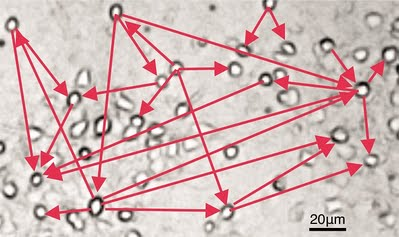
\includegraphics[width=\textwidth]{connectivity.jpg}
    \end{block}
    \end{column}
  \end{columns}
\end{frame}

\begin{frame}{Inferring the Connectome}
\frametitle{What information can we use to infer the connectome?}
  \begin{columns}[T]
    \begin{column}{.5\textwidth}
     \begin{block}{Inferring the Connectome}
\begin{itemize}

\item In wet labs, we can monitor the activity of neurons by placing a fluorescence meter on each neuron. 
\item The hope is to be able to reconstruct the connectome using correlations in this fluorescence data.
\end{itemize}

    \end{block}
    \end{column}
    \begin{column}{.5\textwidth}
    \begin{block}{}
% Your image included here
    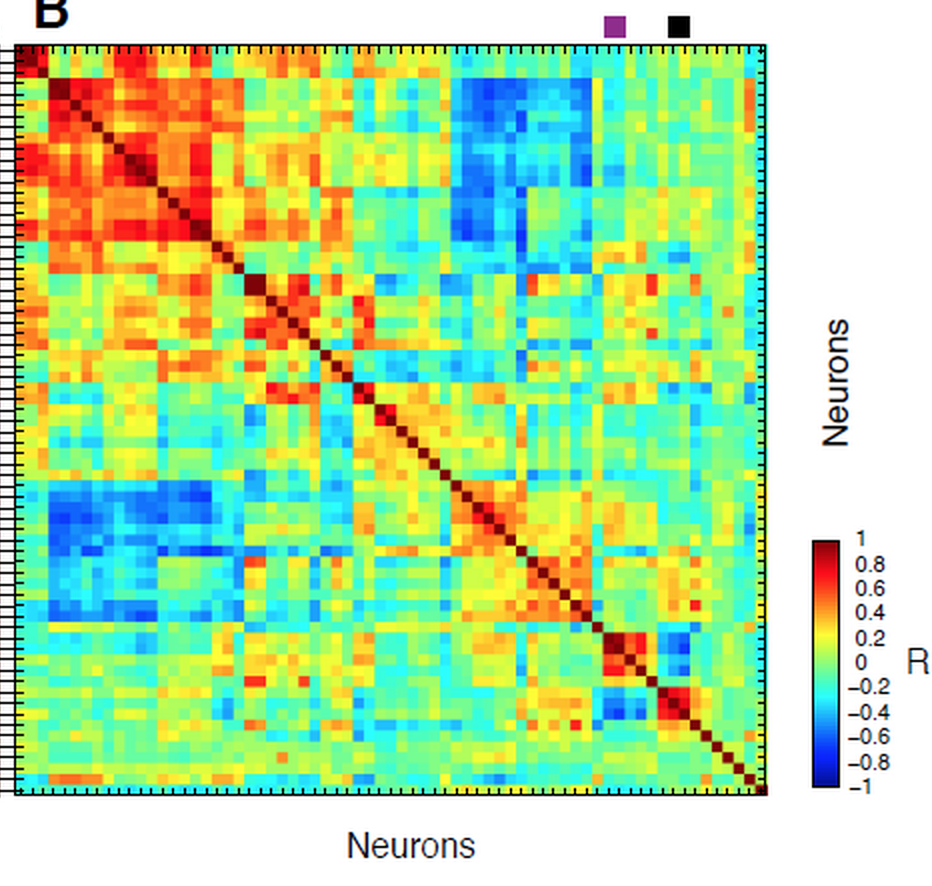
\includegraphics[width=\textwidth]{correlated_neurons.png}
    \end{block}
    \end{column}
  \end{columns}
\end{frame}





\begin{frame}{Stetter 2012}
\begin{itemize}
\item To test the accuracy of a predicted connectome, one needs to know the actual connectome. 
\item Since determining the actual connectome is such a hard problem and consequently very few actual network connectomes are known, the Kaggle challenge uses data simulated from a virtual population of neurons in which the connectome is known via the method outlined in Stetter, 2012\footnote{Stetter O, Battaglia D, Soriano J, Geisel T (2012) Model-Free Reconstruction of Excitatory Neuronal Connectivity from Calcium Imaging Signals. PLoS Comput Biol 8(8): e1002653. doi:10.1371/journal.pcbi.1002653}

\end{itemize}


\end{frame}

\begin{frame}{Latent Variables taken from the Stetter Paper}
\frametitle{Latent Variables taken from the Stetter Paper}
 \begin{columns}[T]
    \begin{column}{.5\textwidth}
   
\begin{block}{Connectivity Constant, $p$}
	The setter paper defines several different latent variables that we incorporated into our simulation. 
	\begin{itemize}
	\item Connectivity constant, $p$, is the chance that two arbitrary neurons are connected to each other. 
	\item This plays into our model in that it affects the prior distribution of what we believe the connectome is. 
	\end{itemize} 

   \end{block}





  
\end{column}
    \begin{column}{36mm}
    \begin{block}{}
% Your image included here
    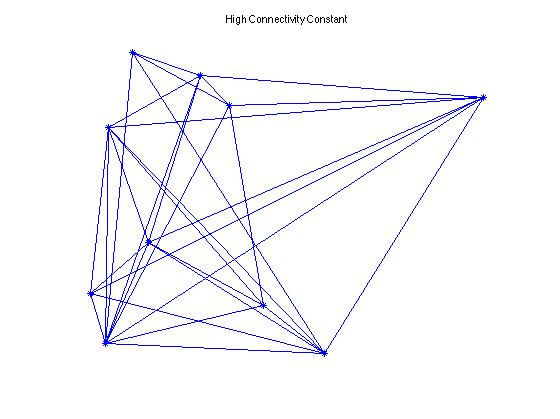
\includegraphics[width=36mm]{high_connectivity_constant.jpg}
   
    \end{block}
    \begin{block}{}
     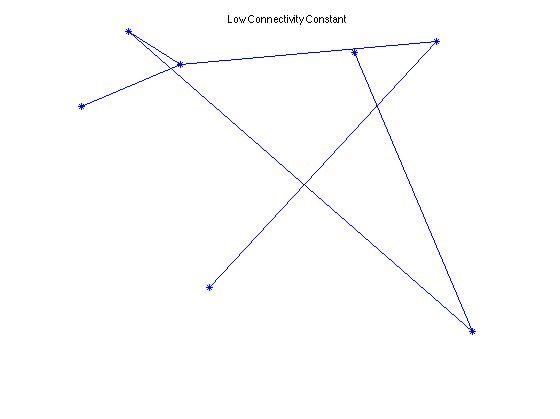
\includegraphics[width=36mm]{low_connectivity_constant.jpg}
     \end{block}
    \end{column}
\end{columns} 


\end{frame}
 
 
 
 
 
 
 
 
 %clustering coefficient 
 \begin{frame}{Latent Variables taken from the Stetter Paper}
\frametitle{Latent Variables taken from the Stetter Paper}
 \begin{columns}[T]
    \begin{column}{.5\textwidth}
   
\begin{block}{Clustering Coefficient}
        $E_{v}/(K_{v}(K_{v}-1)/2)$
	\begin{itemize}
	\item The clustering coefficient is a measure of how tightly the graph "clusters." 
	\item This plays into our model in that it affects the prior distribution of what we believe the connectome is. 
	\end{itemize} 

   \end{block}





  
\end{column}
    \begin{column}{60mm}
    \begin{block}{}
% Your image included here
    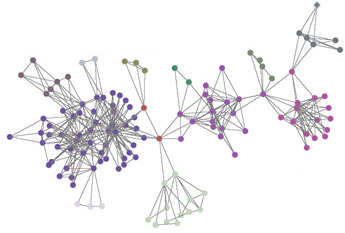
\includegraphics[width=55mm]{high_clustering_coefficient.jpg}
   
    \end{block}
 
    \end{column}
\end{columns} 


\end{frame}
 
 
 
 
 %Data blurring 
 \begin{frame}{Latent Variables taken from the Stetter Paper}
\frametitle{Problems with Fluorescence Data}
 \begin{columns}[T]
    \begin{column}{.5\textwidth}
   
\begin{block}{Fluorescence Blurring}
        
	
	A neuron's fluorescence values effect the fluorescence of other neurons even if they aren't connected due light scattering effects. To the right is an example of an unblurred, "true" fluorescence output from two different neurons. 
   \end{block}





  
\end{column}
    \begin{column}{60mm}
    \begin{block}{}
% Your image included here
    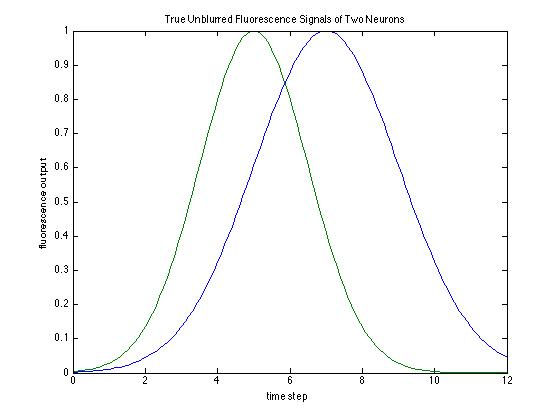
\includegraphics[width=55mm]{two_unblurred_neurons.jpg}
   
    \end{block}
    \end{column}
\end{columns} 

\end{frame}




%Data blurring continued
 \begin{frame}{Latent Variables taken from the Stetter Paper}
\frametitle{Problems  with Fluorescence Data}
 \begin{columns}[T]
    \begin{column}{.5\textwidth}
   
\begin{block}{Fluorescence Blurring}
        
Blurring linearly combines the true fluorescence value of a neuron with the fluorescence values of its neighbors. This causes nearby neural fluorescence data to look more similar than it should. 
   \end{block}





  
\end{column}
    \begin{column}{60mm}
    \begin{block}{}
% Your image included here
    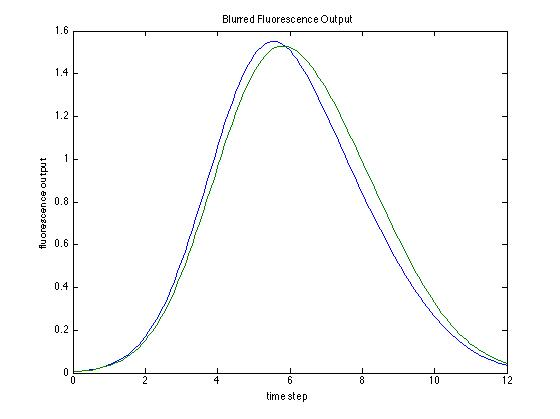
\includegraphics[width=55mm]{blurred_fluorescence.jpg}
   
    \end{block}
    \end{column}
\end{columns} 




\end{frame}


% Too large of time steps to infer which spikes happened first 
 \begin{frame}{Latent Variables taken from the Stetter Paper}
\frametitle{Problems with Fluorescence Data}
  The fluorescence data is sampled in intervals of 20 ms and decays very slowly. The rate of sampling is too slow to infer exactly when spikes happen, and which spikes caused other spikes. 
 \begin{columns}[T]
    \begin{column}{.5\textwidth}
   
    \begin{block}{}
 
% Your image included here
    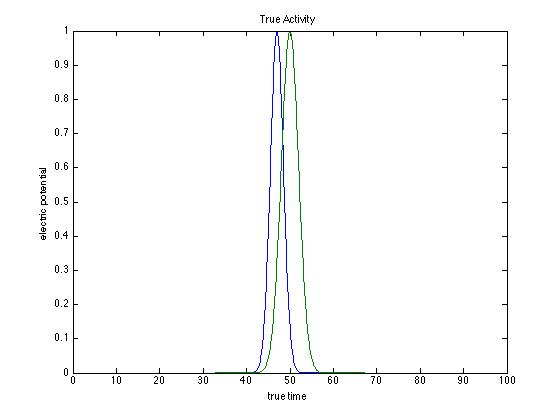
\includegraphics[width=55mm]{true_fluorescence_activity.jpg}
   
    \end{block}
  
\end{column}
    \begin{column}{60mm}

     \begin{block}{}
% Your image included here
    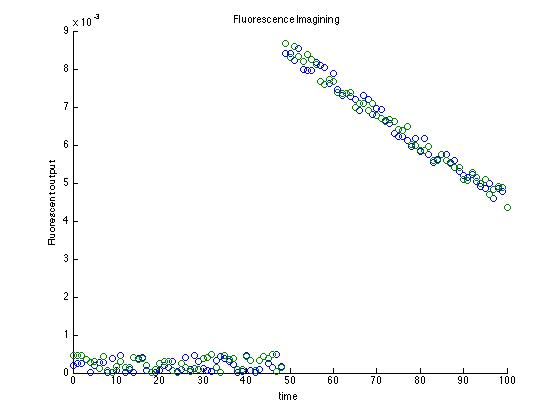
\includegraphics[width=55mm]{fluorescent_timestep_problem.jpg}
   
    \end{block}
    \end{column}
\end{columns} 

\end{frame}

\begin{frame}{Data simulation methods}
\begin{itemize}
\item Stetter 2012 devised a system of differential equations to simulate the fluorescence of interconnected neurons based on a connectome.
\item A connectome was simualted randomly, then connections were altered systematically to create the desired clustering coefficient.
\item Fluorescence values were then blurred to reflect actual systems.
\item The blurred data than had Gaussian noise added, resulting in reported fluorescence values outside [0,1].
\end{itemize}
\end{frame}

\section{Current Approach}

\begin{frame}{General Outline}
\begin{itemize}
\item Set up a Bayesian hierarchical model of the (unspecified) system of differential equations.
\item Use penalization (LASSO and/or Ridge) and "spike and slab" priors to differentiate connection status.
\item Use Markov Chain Monte Carlo (MCMC) (and possibly other methods) to find optimal parameter solutions to the model.
\item Report back MAP and Expectation settings of the Connectome.
\end{itemize}
\end{frame}

\begin{frame}{Statistical Model}
\begin{eqnarray}
C_{ij} & \sim & Bernoulli( \rho ) \\
\beta_{ij} & \sim & N( 0, ( \tau_1 C_{ij} + \tau_0 (1-C_{ij}) ) I ) \\
F_{i,t} & = & N( \left(\begin{smallmatrix} F_{\dot,t-1} \\ F_{i,t-1}F_{\dot,t-1} \end{smallmatrix}\right)^T \beta_i + \epsilon_{i,t}^{\mathbb{M}} \\
F_{i,t}^{bl} & = & A(\alpha, \lambda) F + \epsilon_{i,t}^{\mathbb{B}} \\
A_{ij} &=& \alpha e^{-\frac12 \frac{ || x_i - x_j ||_2^2 }{ \lambda^2 } } + (1 - \alpha) \delta_{i=j}
\end{eqnarray}
\end{frame}

\begin{frame}{Update Rules: C}
\begin{eqnarray}
p( C_{ij} = 1 | \beta_j ) &=& \frac{ \rho N( \beta_{ij} | 0, \tau_1 ) }{ \rho N( \beta_{ij} | 0, \tau_1 ) + (1-\rho) N( \beta_{ij} | 0, \tau_0 )} \\
odds( C_{ij} = 1 | \beta_j  ) & = & \frac{p}{1-p} = \frac{\rho}{1-\rho} \frac{\tau_1}{\tau_0} e^{-\frac12 ||\beta_{ij}||_2^2 ( \tau_1 - \tau_0 ) }\\
\text{Stochastic} & : & \text{Sample } C_{ij} \sim p( C_{ij} = 1 | \beta_j ) \\
\text{MLE} & : & \text{Set } C_{ij} = 1_{ p( C_{ij} = 1 | \beta_j ) > \frac12 }
\end{eqnarray}
\end{frame}

\begin{frame}{Update Rules: $\beta$}

\[ \hat{\beta}_i | C, F  \sim  N\left( (\frac{1}{\sigma^2} X^T X + \tau_{C_i} I)^{-1} \frac{1}{\sigma^2} X^T F, ( \frac{1}{\sigma^2} X^TX + \tau_{C_i} I)^{-1} \right) \]

\begin{itemize}
\item Can easily either sample $\hat{\beta}$ or just use expectation/MLE (center of the Gaussian)
\item Effect of adding $\tau_{C_i} I$ is that filters of disconnected neurons end up being very close to 0, connected neurons end up close to unpenalized MLE. (That is, more shrinkage for disconnected neurons having any effect.)
\item $\sigma^2\tau = \frac{\sigma_{li}^2}{\sigma_{pr}^2} \approx$ signal-to-noise ratio
\item We place a Gamma prior on $1/\sigma^2$ and update using Gibbs sampling of the Gamma posterior.
\end{itemize}

\end{frame}

\begin{frame}{Update Rules: $\alpha, \lambda$}
\begin{itemize}
\item No easy way to optimize or conditionally sample.
\item Return to random-walk metropolis: $\begin{smallmatrix} \alpha' \\ \lambda' \end{smallmatrix} = \begin{smallmatrix} \alpha \\ \lambda \end{smallmatrix} + \epsilon_{2x1}$
\item We sample a series (of arbitrary size) or $\alpha', \lambda'$ pairs centered at $\alpha, \lambda$ and choose either:
\item MLE: $\argmax\limits_{\alpha', \lambda'} p( F^{bl} | A(\alpha',\lambda') \hat{F}, \sigma^2 ) $
\item Expectation: $(\alpha', \lambda') = \sum (\alpha', \lambda') p( F^{bl} | A(\alpha',\lambda') \hat{F}, \sigma^2 ) $
\item Sample: $p(\alpha', \lambda') \propto \sum (\alpha', \lambda') p( F^{bl} | A(\alpha',\lambda') \hat{F}, \sigma^2 )$
\end{itemize}
\end{frame}

\section{Initial Results}

\begin{frame}{How we measured it}
\begin{itemize}
	\item Precision: $\frac{\text{Correct Connections} }{ \text{Total Predicted Connections} } = \frac{ TP }{ FP + TP }$
	\item Recall: $\frac{ \text{Correct Connections} }{ \text{Total True Connections} } = \frac{ TP }{ FN + TP }$
	\item F1 score: $\frac{ 2 * \text{Precision} * \text{Recall} }{ \text{Precision} + \text{Recall} }$
\end{itemize}
\end{frame}

\begin{frame}{Results: 100 neuron network}
\begin{itemize}
\item Note, this network has 100 neurons, and a total of 1050 (10.5\%) non-diagonal connections. We performed stochastic sampling with $\rho = 0.105$.
\end{itemize}

\begin{centering}
\begin{figure}
\begin{tabular}{ c l l l }
Method & Pre & Rec & F1 \\ \hline
All connections & 0.115 & 1.000 & 0.206 \\
Random & 0.115 & 0.182 & 0.141 \\
Result (A) & 0.130 & 0.376 & 0.193 \\
Result (B) & 0.325 & 0.125 & 0.181 \\
\end{tabular}
\end{figure}
\end{centering}

\begin{itemize}
\item Result: We're beating random guessing, but not by a lot.
\end{itemize}
\end{frame}

\begin{frame}{Conclusions}
\begin{itemize}
\item A 2nd-order analysis that looks only 1 timestep back is doing a very poor job.
\item Separating the problems of deblurring and estimating the connectome would be valuable.
\item Higher-order and longer timesteps is trivial to add analytically, but computationally infeasible.
\item Algorithms are highly parallelizable (note $\hat{\beta}_i \perp \hat{\beta}_i$) so may be a good approach in need of serious computing power.
\end{itemize}
\end{frame}

\begin{frame}{Questions?}
Questions?
\end{frame}

\end{document}


